%%%%%%%%%%%%%%%%%%%%%%%%%%%%%%%%%%%%%%%%%
% Template ini dibuat untuk makalah kolokium mahasiswa
% Program Alih Jenis (Ekstensi) Ilmu Komputer IPB
% Version 1.0 (18/05/2015)
%
% Template ini menggunakan template yang di-download dari:
% http://www.LaTeXTemplates.com
% Mathias Legrand (legrand.mathias@gmail.com)
% License: CC BY-NC-SA 3.0 (http://creativecommons.org/licenses/by-nc-sa/3.0/)
%
% Dimodifikasi untuk keperluan Program Studi
% Oleh: JULIO ADISANTOSO (julioipb@gmail.com)
%
% Untuk memudahkan penggunaan, maka diambil contoh makalah atas nama 
% Fithranto Faturakhman di bawah bimbingan Karlisa Priandana ILKOM-IPB.
% Silakan mengganti dan melengkapi file:
%    (1) kolokium_information.tex -- judul, nama, nim, email, pembimbing, dsb
%    (2) abstrak.tex -- abstrak makalah
%    (3) pendahuluan.tex -- berisi latar belakang, dsb
%    (4) metode.tex -- berisi metode penelitian
%    (5) pustaka.bib -- berisi daftar pustaka
%
%%%%%%%%%%%%%%%%%%%%%%%%%%%%%%%%%%%%%%%%%

%----------------------------------------------------------------------------------------
%	PACKAGES AND OTHER DOCUMENT CONFIGURATIONS
%----------------------------------------------------------------------------------------

\documentclass[fleqn,11pt]{SelfArx} % Document font size and equations flushed left
\usepackage[english]{babel}

%----------------------------------------------------------------------------------------
%	COLUMNS
%----------------------------------------------------------------------------------------

\setlength{\columnsep}{0.55cm} % Distance between the two columns of text
\setlength{\fboxrule}{0.75pt} % Width of the border around the abstract

%----------------------------------------------------------------------------------------
%	COLORS
%----------------------------------------------------------------------------------------

\definecolor{color1}{RGB}{0,0,90} % Color of the article title and sections
\definecolor{color2}{RGB}{0,20,20} % Color of the boxes behind the abstract and headings

%----------------------------------------------------------------------------------------
%	HYPERLINKS
%----------------------------------------------------------------------------------------

\usepackage{hyperref} % Required for hyperlinks
\hypersetup{hidelinks,colorlinks,breaklinks=true,urlcolor=color2,citecolor=color1,linkcolor=color1,bookmarksopen=false,pdftitle={Title},pdfauthor={Author}}


%
% Hyphenation untuk Indonesia 
%
% @author  Andreas Febrian
% @version 1.00
% 
% Tambahkan cara pemenggalan kata-kata yang salah dipenggal secara otomatis 
% oleh LaTeX. Jika kata tersebut dapat dipenggal dengan benar, maka tidak 
% perlu ditambahkan dalam berkas ini. Tanda pemenggalan kata menggunakan 
% tanda '-'; contoh: menarik  --> pemenggalan: me-na-rik
%

\hyphenation{
    % alphabhet A
    a-na-li-sa a-tur 
    a-pli-ka-si 
    % alphabhet B
    ba-ngun-an 
    be-be-ra-pa 
    ber-ge-rak
    ber-ke-lan-jut-an 
    ber-pe-nga-ruh 
    Bha-dri-ra-ju
    % alphabhet C
    ca-ri
    % alphabhet D
    di-sim-pan di-pim-pin de-ngan da-e-rah di-ba-ngun da-pat di-nya-ta-kan 
    di-sim-bol-kan di-pi-lih di-li-hat de-fi-ni-si
    % alphabhet E
    e-ner-gi eks-klu-sif
    % alphabhet F
    fa-si-li-tas
    % alphabhet G
    ga-bung-an ge-rak
    % alphabhet H
    ha-lang-an
    % alphabhet I
    % alphabhet J
    jang-krik
    % alphabhet K
    ke-hi-lang-an
    ku-ning 
    kua-li-tas ka-me-ra ke-mung-kin-an ke-se-pa-ham-an
    % alphabhet L
    ling-kung-an
    % alphabhet M
    me-neng-ah me-ning-kat-kan
    meng-a-tas-i me-mung-kin-kan me-nge-na-i me-ngi-rim-kan 
    meng-u-bah meng-a-dap-ta-si me-nya-ta-kan mo-di-fi-ka-si
    meng-a-tur meng-um-pul-kan Men-te-ri
    Mo-ham-med
    % alphabhet N
    nya-ta non-eks-klu-sif
    % alphabhet O
    % alphabhet P
	pe-nye-rap-an 
	pe-ngon-trol
    pe-mo-del-an
    pe-ran  pe-ran-an-nya
    pem-ba-ngun-an pre-si-den pe-me-rin-tah prio-ri-tas peng-am-bil-an 
    peng-ga-bung-an pe-nga-was-an pe-ngem-bang-an 
    pe-nga-ruh pa-ra-lel-is-me per-hi-tung-an per-ma-sa-lah-an 
    pen-ca-ri-an peng-struk-tur-an
    PER-TAM-BANG-AN
    % alphabhet Q
    % alphabhet R
    ran-cang-an
    re-ko-men-da-si
    % alphabhet S
    si-mu-la-si sa-ngat Sa-ma-rin-da
    % alphabhet T
    te-ngah
    ter-da-pat
    % alphabhet U
    % alphabhet V
    % alphabhet W
    % alphabhet X
    % alphabhet Y
    % alphabhet Z
    % special
}
% Tuliskan nama lengkap Anda
\def\namaMhs {Nasrul Hamid (G64164017)\textsuperscript{1}, Muhammad Jaka Utama (G64164021)\textsuperscript{2}, Michael Tampubolon (G64164039)\textsuperscript{3}}

% Tuliskan NIM Anda
%\def\nim {G64164017}

% Tuliskan alamat email Anda
\def\emailMhs {\textsuperscript{1}nasrul\_hamid@apps.ipb.ac.id, \textsuperscript{2}jaka\_utama@apps.ipb.ac.id, \textsuperscript{3}michael\_tampubolon@apps.ipb.ac.id }

% Tuliskan nama lengkap dosen pembimbing
\def\namaDosen {Yeni Herdiyeni}

% Tuliskan judul makalah kolokium di definisi "judul"
\def\judul {Pendeteksian Rintangan bagi Penyandang Tuna Netra}

% Tuliskan kata kunci, dipisahkan oleh tanda titik-koma
\def\katakunci {estimasi jarak; pendeteksian objek; penginderaan komputer}


\usepackage{xcolor,colortbl}
\usepackage{multicol}
\usepackage{multirow}
\usepackage{graphicx,xcolor}
\graphicspath{{gambar/}}

\usepackage[urldate=comp, backend=biber, style=authoryear, url=true, doi=true, maxbibnames=4, maxcitenames=2, block=none, sorting=nyt]{biblatex}
\usepackage{xpatch}
\addbibresource{pustaka.bib}
\DefineBibliographyStrings{english}{%
	and = {dan}
}
\DefineBibliographyStrings{english}{%
	andothers = {\em et\addabbrvspace al\adddot}
}
\renewbibmacro{in:}{
	\iffieldundef{journaltitle}
	{}
	{\xspace dalam:}
}
\renewbibmacro*{volume+number+eid}{%
	\printfield{volume}%
	%  \setunit*{\adddot}% DELETED
	\setunit*{\addnbspace}% NEW (optional); there's also \addnbthinspace
	\printfield{number}%
	\setunit{\addcomma\space}%
	\printfield{eid}}
\DeclareFieldFormat[article]{number}{\mkbibparens{#1}}
\DeclareFieldFormat{url}{\printtext{Dapat diunduh dari}\addcolon\space\url{#1}}
%\DeclareFieldFormat{urldate}{#1}
\DeclareFieldFormat{urldate}{%
	\thefield{urlday}\addslash%
	\thefield{urlmonth}\addslash%
	\thefield{urlyear}\isdot}

\renewbibmacro*{url+urldate}{%
	\iffieldundef{urlyear}
	{}
	{\setunit*{\addspace}%
		\printtext{[Internet]. [}%
		\printtext{Diunduh tanggal}\space%
		\printurldate\space
		\printtext{].}\space%
		\printfield{url}}%
}
\xpatchbibmacro{date+extrayear}{%
  \printtext[parens]%
}{%
  \setunit{\addperiod\space}%
  \printtext%
}{}{}
\nocite{*}


%\usepackage[urldate=iso8601, backend=biber, style=authoryear, url=true, doi=true, sorting=nyt]{biblatex}
%\addbibresource{pustaka.bib}
%\DefineBibliographyStrings{english}{%
%	urlseen = {diunduh pada},
%}
%\renewbibmacro{in:}{\xspace dalam:}
%\renewbibmacro*{volume+number+eid}{%
%	\printfield{volume}%
%	%  \setunit*{\adddot}% DELETED
%	\setunit*{\addnbspace}% NEW (optional); there's also \addnbthinspace
%	\printfield{number}%
%	\setunit{\addcomma\space}%
%	\printfield{eid}}
%\DeclareFieldFormat[article]{number}{\mkbibparens{#1}}

%----------------------------------------------------------------------------------------
%	ARTICLE INFORMATION
%----------------------------------------------------------------------------------------

\JournalInfo{Projek Akhir Pengenalan Citra Digital (KOM324)} % Journal information
\Archive{Departemen Ilmu Komputer, FMIPA-IPB} % Departemen ILKOM-IPB

\PaperTitle{\judul} 

%\Authors{\namaMhs, \namaDosen} % Penulis
\Authors{\namaMhs} % Penulis
\affiliation{\scriptsize\textbf{Alamat Email}: \emailMhs \normalsize} % Corresponding author

\Keywords{\scriptsize \katakunci \normalsize} 
\newcommand{\keywordname}{Kata Kunci} % Defines the keywords heading name

%----------------------------------------------------------------------------------------
%	ABSTRACT
%----------------------------------------------------------------------------------------
\Abstract{\scriptsize 
% ---- Tuliskan abstrak di bagian ini seperti contoh.
	%Latarbelakang
	Kemampuan untuk mengenali dan mengidentifikasi lingkungan sangat dibutuhkan setiap individu untuk dapat berinteraksi dengan benar. Penyandang tuna netra kerap mengalami kesulitan untuk menghindari rintangan dan menemukan lajur yang benar.
	%tujuan & %metode
	Salah satu pendekatan sebagai alternatif adalah pemanfaatan pengolahan citra digital dalam pengidentifikasian lajur, jenis rintangan, dan estimasi jarak. Solusi diharapkan dapat memberikan beberapa pertimbangan yang komprehensif.
% ---- Akhir bagian abstrak
\normalsize}


%----------------------------------------------------------------------------------------

\begin{document}

\flushbottom % Makes all text pages the same height

\maketitle % Print the title and abstract box

\thispagestyle{empty} % Removes page numbering from the first page

%----------------------------------------------------------------------------------------
%	BAGIAN PENDAHULUAN
%----------------------------------------------------------------------------------------

%----------------------------------------------------------------------------------------
%	PENDAHULUAN
%----------------------------------------------------------------------------------------
\section*{PENDAHULUAN} % Sub Judul PENDAHULUAN
% Tuliskan isi Pendahuluan di bagian bawah ini. 
% Jika ingin menambahkan Sub-Sub Judul lainnya, silakan melihat contoh yang ada.
% Sub-sub Judul 
\subsection*{Latar Belakang}
Setiap individu selalu berinteraksi terhadap lingkungan dalam setiap aktivitasnya. Salah satunya saat berjalan, manusia umumnya mengidentifikasi objek di sekitarnya sebelum menentukan arah geraknya. Hal ini kerap menjadi kesulitan bagi beberapa orang utamanya penyandang tuna netra.


Salah satu pendekatan yang dapat dilakukan adalah dengan pemanfaatan teknologi penginderaan komputer \textit{(computer vision)}. \citeauthor{rajput2014smart} (\cite*{rajput2014smart}) telah meneliti dan mengembangkan \textit{Smart Object Detector (SOD)} berupa tongkat yang menggunakan software MATLAB untuk memproses video secara efisien dan cepat untuk mendeteksi objek, mengkombinasikannya dengan sensor ultrasonik untuk mengukur jarak objek kemudian mengkonversinya menjadi suara dan getaran.

\citeauthor{Yi2013} (\cite*{Yi2013}) mengumpulkan data objek yang kerap dijumpai dan mengaplikasikan \textit{Speeded-Up Robust
Features and Scale Invariant Feature Transform (SURF/SIFT)} pada citra-citra yang dibagikan sekumpulan kamera dalam sistem jaringan untuk mengenali objek-objek tersebut.

\citeauthor{wang2014rgb} (\cite*{wang2014rgb}) mengimplementasi transformasi Hough pada kanal RGB untuk mengekstraksi garis-garis paralel citra sebagai fitur identifikasi tangga dan penyeberangan \textit{zebra cross}. Objek tangga kemudian dibedakan ke dalam tangga naik dan tangga turun menggunakan pengklasifikasian SVM.

Penelitian ini bertujuan untuk membuat alat pendeteksi rintangan bagi pejalan kaki utamanya penyandang tuna netra menggunakan kamera tunggal sebagai input, dan suara sebagai output. Output dapat berupa nada \textit{low tone} yang bervariasi berdasarkan jenis objek dan estimasi jarak.

% Sub-sub Judul 
\subsection*{Tujuan}

Tujuan dari penelitian ini adalah:
\begin{enumerate}[noitemsep] 
\item Membuat prototipe software pendeteksi rintangan dan lajur pejalan kaki.
\item Mengukur akurasi pengenalan objek.
\end{enumerate}

\subsection*{Ruang Lingkup}

Ruang lingkup penelitian adalah:
\begin{enumerate}[noitemsep] 
\item Lokasi pengujian memiliki intensitas cahaya minimal 100 lux.
\item Objek yang diidentifikasi diklasifikasikan ke dalam objek umum seperti manusia, tangga, dan pintu. Objek selainnya dikelompokkan ke dalam objek bergerak dan objek diam.
\item Output suara berupa \textit{tone} rendah yang bervariasi berdasarkan jenis dan estimasi jarak.
\item Produk yang dihasilkan adalah berupa prototipe program komputer.
\end{enumerate}

\subsection*{Manfaat}

Hasil penelitian diharapkan dapat membantu pejalan kaki terutama penyandang tuna netra untuk dapat meningkatkan kewaspadaan dan sebagai pemandu saat berjalan.

%----------------------------------------------------------------------------------------
%	BAGIAN METODE
%----------------------------------------------------------------------------------------

%----------------------------------------------------------------------------------------
%	METODE
%----------------------------------------------------------------------------------------
\section*{METODE PENELITIAN}
Penelitian yang dilakukan terbagi menjadi beberapa tahapan proses. 
\iffalse
Gambar \ref{fig:tahapan} menunjukan tahapan proses tersebut.

\begin{figure}[h!] % Gunakan \begin{figure*} untuk memasukkan Gambar
\centering
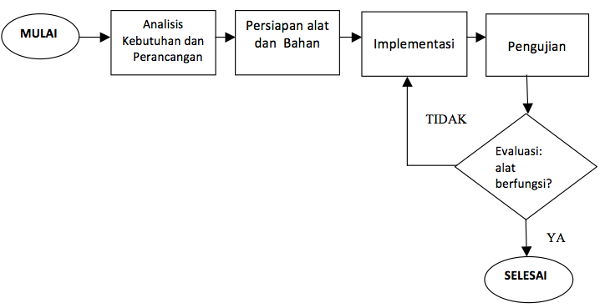
\includegraphics[width=200pt]{kolokium_contoh_gb1.png}
\caption{Tahapan proses penelitian}
\label{fig:tahapan}
\end{figure}
\fi
\subsection*{Analisa Kebutuhan dan Perancangan}

Komponen utama yang akan digunakan pada penelitian adalah komputer / laptop dengan dukungan OpenCV dan kamera digital. Gambar \ref{fig:alat} merupakan ilustrasi dari alat yang akan dibuat.

\begin{figure}[h!]\centering % Gunakan \begin{figure*} untuk memasukkan Gambar
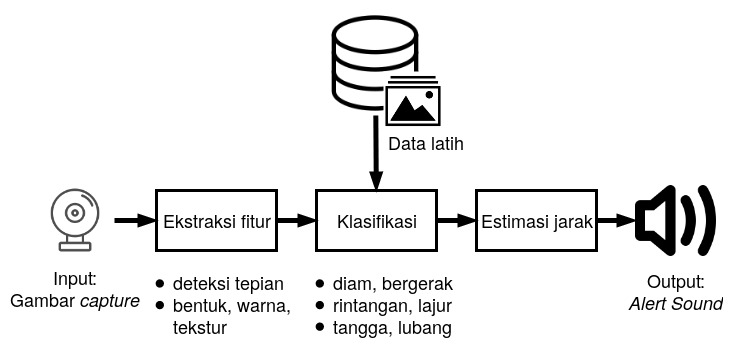
\includegraphics[width=\columnwidth]{prototipe-obstacle-detector}
\caption{Ilustrasi prototipe}
\label{fig:alat}
\end{figure}

\subsection*{Persiapan Alat dan Bahan}

Kegiatan yang dilakukan pada tahap ini adalah mengumpulkan alat dan bahan yang akan digunakan pada penelitian, yakni:
\begin{enumerate}
	\item Komputer dengan dukungan OpenCV dan C++
	\item Kamera portable yang dapat dikoneksikan dengan komputer untuk \textit{live video} atau dapat pula menggunakan file video yang direkam sebelumnya.
	\item Persiapan data latih yang akan digunakan untuk pengenalan objek dan klasifikasi. Pada tahapan ini software yang digunakan adalah RStudio.
\end{enumerate}

\subsection*{Implementasi}

Pada tahap ini dikembangkan produk berupa prototipe program berbasis C++ mennggunakan library OpenCV.

\subsection*{Pengujian dan Evaluasi}

Pengujian dilakukan untuk mengukur akurasi hasil pengenalan objek. Aplikasi berusaha:
\begin{enumerate}
	\item mendeteksi objek yang telah didefinisikan, di antaranya: pejalan kaki, kendaraan, dan pintu
	\item objek yang tidak dikenal dikategorikan menjadi objek diam, atau objek bergerak. 
	\item memperkirakan estimasi jarak dari posisi pengguna ke posisi objek.
	\item jangkauan deteksi adalah maksimal 10 meter di depan kamera.
	\item Output berupa \textit{tone} rendah dengan beberapa variasi frekuensi dan tempo untuk membedakan jenis objek dan estimasi jarak.
\end{enumerate}

\iffalse
\subsection*{Evaluasi}

Pengujian yang dilakukan di tahap sebelumnya dievaluasi pada tahap ini. Pengujian pertama dinyatakan berhasil jika efisiensi frekuensi mencapai 100$\%$ artinya frekuensi yang dihasilkan sesuai dengan input yang dimasukkan. Pengujian kedua dinyatakan berhasil jika tikus yang berada pada kandang berpindah tempat ke kandang lain setelah terkena gelombang ultrasonik dari alat. Pengulangan implementasi dilakukan jika salah satu atau kedua pengujian dinyatakan tidak berhasil atau gagal.
\fi
\subsection*{Jadwal Kegiatan}

Penelitian ini akan dilakukan dalam 5 pekan dengan rincian kegiatan seperti tercantum pada Tabel \ref{tab:jadwal}.
\begin{table}[t!]
	\begin{center}
		\caption{Rencana Jadwal Penelitian}
		\label{tab:jadwal}
		\footnotesize
		\begin{tabular}{|l|c|c|c|c|c|}
			\hline
			\iffalse
			\multirow{2}{*}{Kegiatan}&\multicolumn{2}{c|}{1}&\multicolumn{4}{c|}{2}&\multicolumn{4}{c|}{3}&\multicolumn{4}{c|}{4}&\multicolumn{4}{c|}{5}\\
			\cline{2-19}
			\fi
			Kegiatan&1&2&3&4&5\\
			\hline \hline
			Persiapan alat dan bahan &\cellcolor{black}&&&&\\
			\hline
			Penyusunan data latih&&\cellcolor{black}&\cellcolor{black}&&\\
			\hline
			Implementasi&&&\cellcolor{black}&\cellcolor{black}&\\
			\hline
			Pengujian dan Evaluasi&&&&\cellcolor{black}&\cellcolor{black}\\
			\hline
		\end{tabular}
		\normalsize
	\end{center}
\end{table}

\iffalse
\subsection*{Contoh Penulisan}

Bagian ini sengaja diisi dengan beberapa contoh penulisan dalam LaTex untuk memudahkan menulis makalah dengan cepat menggunakan LaTex. Berikut adalah contoh membuat tabel yang dapat dirujuk. Misalnya, Tabel \ref{tab:daftarsaya} menjelaskan sesuatu yang terkait dengan naskah ini.

\begin{table}[hbt]
\caption{Daftar Nilai}
\centering
\begin{tabular}{llr}
\toprule
\multicolumn{2}{c}{Name} \\
\cmidrule(r){1-2}
First name & Last Name & Grade \\
\midrule
John & Doe & $7.5$ \\
Richard & Miles & $2$ \\
\bottomrule
\end{tabular}
\label{tab:daftarsaya}
\end{table}

Kadangkala kita juga perlu menuliskan suatu formula matematika dalam sebuah kalimat. Misalnya, ada formula matematika $\cos^3 \theta =\frac{1}{4}\cos\theta+\frac{3}{4}\cos 3\theta$, dimana penulisan formula ini berbeda dengan formula sebelumnya yang diberi referensi atau nomor formula yang dapat diacu di dalam sebuah teks kalimat.

Tabel \ref{tab:tag} menunjukkan contoh suatu tabel yang memiliki lebar melebihi kolom yang diinginkan, sehingga perlu diatur lebar sesuai yang diinginkan. Dalam hal ini digunakan paket \textit{tabulary}.

\begin{table}[h!]
\footnotesize
\caption{Deskripsi dokumen XML tanaman obat}
\centering
\begin{tabulary}{0.45\textwidth}{LL}
\toprule
\parbox{12em}{Nama Tag} & Deskripsi \\
\midrule
$<$dok$>$&Mewakili keseluruhan dokumen\\
$<$id$>$&Menjelaskan id dokumen\\
$<$nama$>$&Nama tanaman obat\\
$<$namal$>$&Nama latin tanaman obat\\
$<$deskripsi$>$&Deskripsi tanaman obat yang terdiri dari manfaat, habitus, bagian yang digunakan dan kandungan zat kimia\\
$<$fam$>$&Famili tanaman obat\\
$<$penyakit$>$&Penyakit yang dapat disembuhkan oleh tanaman obat.\\
\bottomrule
\end{tabulary}
\label{tab:tag}
\end{table}

\subsection*{Contoh Penulisan Algoritme}
Algoritme \ref{algo:max} dibuat untuk mendapatkan bilangan terbesar dari kumpulan bilangan yang terhingga.

\begin{algorithm}
\DontPrintSemicolon % Some LaTeX compilers require you to use \dontprintsemicolon instead
\KwIn{Himpunan $A=\{a_1, a_2, \ldots, a_n\}$}
\KwOut{Bilangan terbesar}
$max \gets a_1$\;
\For{$i \gets 2$ \textbf{to} $n$} {
  \If{$a_i > max$} {
    $max \gets a_i$\;
  }
}
\Return{$max$}\;
\caption{{\sc Max} mendapatkan bilangan terbesar}
\label{algo:max}
\end{algorithm}
\fi

%----------------------------------------------------------------------------------------
%	BAGIAN DAFTAR PUSTAKA
%----------------------------------------------------------------------------------------

\renewcommand{\refname}{DAFTAR PUSTAKA}
\nocite{*}
\printbibliography

%----------------------------------------------------------------------------------------

\end{document}